% Paquets généraux
\documentclass[a4paper,12pt,titlepage]{article}
\usepackage[T1]{fontenc}
\usepackage[utf8]{inputenc}
\usepackage[french]{babel}
\usepackage[gen]{eurosym}
%\usepackage[dvips]{graphicx}
\usepackage{fancyhdr}
\usepackage{pdfpages} 
\usepackage{multido}
\usepackage{moreverb}
\usepackage{hyperref}
%\usepackage{textcomp}
\usepackage{verbatim}
\usepackage{moreverb}
\usepackage{listings}
\usepackage{minted}
\usepackage{eso-pic}
\usepackage{enumitem}
\usepackage{comment}
\usepackage{boxedminipage}
\usepackage[french,onelanguage, boxruled,linesnumbered]{algorithm2e}


\newcommand{\auteurun}{Juliette Genzmer}
\newcommand{\auteurdeux}{Willie Robert}
\newcommand{\auteurtrois}{Renaud Costadoat}
\newcommand{\institute}{Lycée Dorian}
\newtheorem{solution}{Solution}


\newcommand{\nom}{Retouche d'images}
\newcommand{\sequence}{1}
\newcommand{\numero}{03}
\newcommand{\type}{DS}
\newcommand{\descrip}{Retouche d'images}


\usepackage{color}
\usepackage{xcolor}
\usepackage{colortbl}
\usepackage{helvet}
\renewcommand{\familydefault}{\sfdefault}
\usepackage{amsfonts}
\usepackage{amsmath}
%\usepackage{xspace}
\usepackage{varioref}
\usepackage{tabularx}
%\usepackage{floatflt}
\usepackage{graphics}
\usepackage{wrapfig}
\usepackage{textcomp}
\usepackage{tikz}
\usepackage{wrapfig}
\usepackage{gensymb}
\usepackage{ifthen}
\usepackage{cancel}
\usepackage{etoolbox}
\usepackage{multirow}
%\usepackage{boxedminipage}
\definecolor{gris25}{gray}{0.75}
\definecolor{bleu}{RGB}{18,33,98}
\definecolor{bleuf}{RGB}{42,94,171}
\definecolor{bleuc}{RGB}{231,239,247}
\definecolor{rougef}{RGB}{185,18,27}
\definecolor{rougec}{RGB}{255,188,204}%255,230,231
\definecolor{vertf}{RGB}{103,126,82}
\definecolor{vertc}{RGB}{220,255,191}
\definecolor{forestgreen}{rgb}{0.13,0.54,0.13}
\definecolor{blcr}{rgb}{0.59,0.69,0.84}
\definecolor{blfr}{rgb}{0.32,0.51,0.75}
\definecolor{orfr}{rgb}{0.90,0.42,0.15}
\definecolor{orcr}{rgb}{0.90,0.65,0.50}
\definecolor{orangef}{rgb}{0.659,0.269,0.072}
\definecolor{orange}{rgb}{0.58,0.35,0.063}
\definecolor{orangec}{rgb}{0.43,0.32,0.25}
\definecolor{rcorrect}{rgb}{0.6,0,0}
\definecolor{sequence}{rgb}{0.75,0.75,0.75}
\definecolor{competences}{rgb}{0.61,0.73,0.35}
\definecolor{grisf}{HTML}{222222}
\definecolor{grisc}{HTML}{636363}
\definecolor{normal}{HTML}{4087c4}
\definecolor{info}{HTML}{5bc0de}
\definecolor{success}{RGB}{92,184,92}
\definecolor{warning}{RGB}{240,173,78}
\definecolor{danger}{RGB}{217,83,79}
\hypersetup{                    % parametrage des hyperliens
    colorlinks=true,                % colorise les liens
    breaklinks=true,                % permet les retours à la ligne pour les liens trop longs
    urlcolor= blfr,                 % couleur des hyperliens
    linkcolor= orange,                % couleur des liens internes aux documents (index, figures, tableaux, equations,...)
    citecolor= forestgreen                % couleur des liens vers les references bibliographiques
    }

% Mise en page
\pagestyle{fancy}

\setlength{\hoffset}{-18pt}

\setlength{\oddsidemargin}{0pt} 	% Marge gauche sur pages impaires
\setlength{\evensidemargin}{0pt} 	% Marge gauche sur pages paires
\setlength{\marginparwidth}{00pt} 	% Largeur de note dans la marge
\setlength{\headwidth}{481pt} 	 	% Largeur de la zone de tête (17cm)
\setlength{\textwidth}{481pt} 	 	% Largeur de la zone de texte (17cm)
\setlength{\voffset}{-18pt} 		% Bon pour DOS
\setlength{\marginparsep}{7pt}	 	% Séparation de la marge
\setlength{\topmargin}{-30pt} 		% Pas de marge en haut
\setlength{\headheight}{55pt} 		% Haut de page
\setlength{\headsep}{20pt} 		% Entre le haut de page et le texte
\setlength{\footskip}{30pt} 		% Bas de page + séparation
\setlength{\textheight}{700pt} 		% Hauteur de l'icone zone de texte (25cm)
\setlength\fboxrule{1 pt}
\renewcommand{\baselinestretch}{1}
\setcounter{tocdepth}{1}
\newcommand{\cadre}[2]
{\fbox{
  \begin{minipage}{#1\linewidth}
   \begin{center}
    #2\\
   \end{center}
  \end{minipage}
 }
}

\newcounter{num_quest} \setcounter{num_quest}{0}
\newcounter{num_rep} \setcounter{num_rep}{0}
\newcounter{num_cor} \setcounter{num_cor}{0}

\newcommand{\question}[1]{\refstepcounter{num_quest}\par
~\ \\ \parbox[t][][t]{0.15\linewidth}{\textbf{Question \arabic{num_quest}}}\parbox[t][][t]{0.85\linewidth}{#1\label{q\the\value{num_quest}}}\par\par
}



\newcommand{\reponse}[0]{\refstepcounter{num_rep}\par
~\ \\ \parbox[t][][t]{0.15\linewidth}{\textbf{Question \arabic{num_rep}}}}

\newcommand{\cor}
{\refstepcounter{num_cor}
\noindent
\rule{\linewidth}{.5pt}
\textbf{Question \arabic{num_cor}:} \\
}



% En tête et pied de page
\lhead{\nom}
\rhead{
\includegraphics[width=2cm]{../../../img/logo}}
\lfoot{David Aubert, Renaud Costadoat}
\rfoot{Page \thepage}
\cfoot{}

\newlength{\RoundedBoxWidth}
\newsavebox{\GrayRoundedBox}
\newenvironment{GrayBox}[1][\dimexpr\textwidth-4.5ex]%
   {\setlength{\RoundedBoxWidth}{\dimexpr#1}
    \begin{lrbox}{\GrayRoundedBox}
       \begin{minipage}{\RoundedBoxWidth}}%
   {   \end{minipage}
    \end{lrbox}
    \begin{center}
    \begin{tikzpicture}%
       \draw node[draw=bleuf,fill=bleuc,rounded corners,%
             inner sep=2ex,text width=\RoundedBoxWidth]%
             {\usebox{\GrayRoundedBox}};
    \end{tikzpicture}
    \end{center}}

\fancypagestyle{correction}{%
  \fancyhf{}
  \lhead{\colorbox{danger}{\begin{minipage}{0.65\paperwidth} \textcolor{white}{\textbf{Correction}} \end{minipage}} }
  \rhead{
\includegraphics[width=2cm]{../../../img/logo}}
  \lfoot{Juliette Genzmer, Willie Robert, Renaud Costadoat}
  \rfoot{\colorbox{danger}{\begin{minipage}{0.3\paperwidth} \begin{flushright}\textcolor{white}{\textbf{Correction}}\end{flushright} \end{minipage}} }}

\renewcommand{\footrulewidth}{0.4pt}


\newcommand{\BackgroundPic}{%
\put(0,0){%
\parbox[b][\paperheight]{\paperwidth}{%
\vfill
\begin{center}
\hspace{0.5cm}\vspace{0.5cm}

\includegraphics[width=\paperwidth,height=\paperheight,%
keepaspectratio]{../../../img/fond5}%
\end{center}
\vfill
}}}

\newcommand{\goforum}{
\begin{figure}[ht!]
\begin{center}
 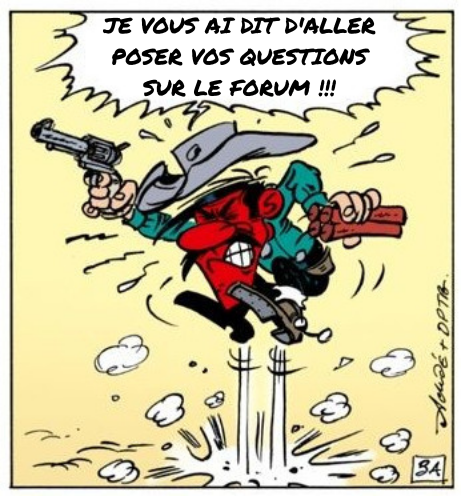
\includegraphics[width=0.7\linewidth]{../../../img/go_forum}
\end{center}
\label{go_forum}
\caption{J'pète les plombs}
\end{figure}}

\newcommand{\BackgroundPicdeux}{%
\put(25,-30){%
\parbox[b][\paperheight]{\paperwidth}{%
\vfill
\begin{center}

\includegraphics[width=\paperwidth,height=\paperheight,%
keepaspectratio]{../../../img/fond6}%
\end{center}
\vfill
}}}

\setenumerate[1]{align=left,label=\arabic*}
\setenumerate[2]{before=\stepcounter{enumi},label*=.\arabic*,leftmargin=1.2em,align=left}

\begin{document}


\pagestyle{fancy}

\AddToShipoutPicture{\BackgroundPicdeux}

\begin{center}
{\Large\bf {\type} \no {\numero} -- \descrip}
\end{center}

\SetKw{KwFrom}{de} 

\begin{boxedminipage}{.9\textwidth} 
\begin{itemize}
 \item Faire tous les exercices dans un fichier {NomPrenom.py} à sauvegarder,
 \item mettre en commentaire l'exercice et la question traités (ex: \# Exercice 1),
 \item ne pas oublier pas de commenter ce qui est fait dans votre code (ex: \# Je crée une fonction pour calculer la racine d'un nombre),
 \item il est possible de demander un déblocage pour une question, mais celle-ci sera notée 0,
 \item il faut vérifier avant de partir que le code peut s'exécuter et qu'il affiche les résultats que vous attendez. Les lignes de code qui doivent s'exécuter sont décommentées.
\end{itemize}
\end{boxedminipage}

\title{Devoir d'informatique en Python \\ \large Simulation d’un distributeur automatique}

\section*{Contexte}
L'objectif de cette étude est de retoucher, à l'aide d'un script Python, une image en jouant sur la luminosité, le contraste et l'effet Bokeh (qui consiste à rendre flou l'arrière plan).

Le portrait que nous allons utiliser pour cette étude est celui de la Joconde de Léonard de Vinci, présent dans le dossier \og Ressources\ \fg sous le nom \og mona\_lisa.png \fg.

\section{Import d'une image et modifications de base}

\subsection{Charger et afficher une image}

\question{\textbf{Copier} le code suivant pour charger l'image et y \textbf{ajouter} la commande \verb?shape? afin d'afficher ses dimensions.}
 
\begin{minted}{python}
import numpy as np
import matplotlib.pyplot as plt
import matplotlib.image as img

img = img.imread("mona_lisa.png")
\end{minted}

\question{\textbf{Afficher} l'image à l'aide des commandes \verb?imshow(img)? et \verb?show()? de la bibliothèque \verb?matplotlib?.}

\subsection{Modifier une image}

Nous allons dans la suite jouer sur la luminosité et le contraste de cette image.

Pour modifier ces paramètres, il faut appliquer la formule suivante à chaque valeur de couleur de chaque pixel: \verb?valeur=contraste*valeur+luminosite?, avec 
\verb?contraste? et \verb?luminosite? des valeurs à modifier selon le réglage souhaité.

Attention, il faut veiller à ce que la valeur issue de ce calcul soit toujours comprise entre 0 et 1, sinon il y a aura une erreur à l'exécution. Pour cela, il faut utiliser la fonction \verb?clip? de la bibliothèque \verb?numpy?.

\question{\textbf{Créer} une fonction \texttt{contraste\_luminosite(image,contraste,luminosite)} qui permet de modifier le contraste et la luminosité de l'image. \textbf{Copier} le code suivant pour la mettre en \oe uvre.}

\begin{minted}{python}
def contraste_luminosite(image,contraste,luminosite):
    ...

f, axarr = plt.subplots(1,2)
axarr[0].imshow(img)
axarr[0].set_title("Image originale")
axarr[0].axis('off')

axarr[1].imshow(contraste_luminosite(img,2,-0.5))
axarr[1].set_title("Nouvelle image")
axarr[1].axis('off')
plt.show()
\end{minted}

\section{Effet Bokeh numérique}

\subsection{Isoler l'arrière plan du sujet}

L’objectif de cette partie est de mettre en valeur le sujet principal, Mona Lisa, en appliquant un flou à l’arrière-plan, tout en laissant le sujet net.

Pour cela, nous utiliserons un masque binaire. Ce masque a la forme d'une liste contenant, pour chaque pixel de l'image, la valeur :
\begin{itemize}
 \item 1 si c'est un pixel du sujet (zone à laisser nette),
 \item 0 si c'est un pixel de l’arrière-plan (zone à flouter).
\end{itemize}

Ce masque est disponible dans le fichier \og masque\_mona\_lisa.csv \fg, le séparateur de colonne utilisé ici est \og,\fg.

\question{\textbf{Importer} ce masque en créant une liste \verb?mask? qui contient les valeurs du masque. \textbf{Afficher} la valeur de \verb?mask[40]?.}

\subsection{Floutage de l'arrière plan}

Dans la suite, il faut implémenter le flou. Cela revient à appliquer plusieurs fois un filtre moyenneur 3x3 sur chaque pixel. Ce flou moyenneur revient à remplacer la valeur d'un pixel par la moyenne des 9 pixels voisins (lui inclus) dans une fenêtre 3x3 centrée sur lui :

~\ \\

\begin{minipage}{0.45\linewidth}
\[
I'(i,j)
=
\frac{1}{9}
\sum_{k=-1}^{1}
\sum_{l=-1}^{1}
I(i+k, j+l)
\]
\end{minipage}\hfill
\begin{minipage}{0.45\linewidth}
\renewcommand{\arraystretch}{2}  % facteur multiplicatif
\begin{tabular}{|c|c|c|}
\hline
I(i-1,j-1) & I(i-1,j) & I(i-1,j+1)\\
\hline
I(i,j-1) & I(i,j) & I(i,j+1)\\
\hline
I(i+1,j-1) & I(i+1,j) & I(i+1,j+1)\\
\hline
\end{tabular}
\renewcommand{\arraystretch}{1}  % remettre à la valeur par défaut
\end{minipage}

~\

Rappel $I(i,j)=[R_{(i,j)},G_{(i,j)},B_{(i,j)}]$ est un vecteur dont les composantes représentent les valeurs des couleurs Rouge, Vert, Bleu du pixel.

\question{\textbf{Coder} la fonction \texttt{moyenne\_voisins(img,i,j)} qui permet de calculer cette moyenne.}

\texttt{moyenne\_voisins(img,75,11)} doit renvoyer \verb?[0.3381264  0.28496733 0.18649238]?.

~\

En appliquant cette opération plusieurs fois :
\begin{itemize}
 \item les détails fins de l’arrière-plan disparaissent progressivement,
 \item l’effet de flou devient plus prononcé,
 \item le sujet principal reste net grâce au masque.
\end{itemize}

Le code suivant permet d'appliquer le flou sur l'arrière plan de la Joconde.

\begin{minted}{python}
def flou(img, n):
    img_blur = img.copy()
    h, w = img.shape[:2]
    for iter in range(n):
        for i in range(1,h-1):
            for j in range(1,w-1):
                if mask[i,j]==.....:
                    img_blur[i,j] = moyenne_voisins(img,i,j)
    return img_blur

fig, axes = plt.subplots(1, 2)
axes[0].imshow(img)
axes[0].set_title("Image originale")
axes[0].axis('off')
axes[1].imshow(flou(img, n=2))
axes[1].set_title("Arrière-plan flou")
axes[1].axis('off')
plt.show()
\end{minted}

\question{\textbf{Remplacer} les \verb?.....? dans le code afin que l'effet Bokeh soit appliqué sur l'arrière plan de l'image.}

\question{\textbf{Créer} une fonction \texttt{flou\_recursif(img, n)} qui effectue le mettre travail que la fonction \texttt{flou(img, n)} mais en utilisant un algorithme récursif. \textbf{Afficher} l'image obtenue par cette nouvelle fonction.}

\begin{center}
FIN
\end{center}
 
\cleardoublepage

\ifdef{\public}{\end{document}}{\pagestyle{correction}}

\begin{center}
\Large{Correction}
\end{center}

\reponse{}

\begin{minted}{python}
import numpy as np
import matplotlib.pyplot as plt
import matplotlib.image as img

img = img.imread("mona_lisa_l.png")
print(img.shape)
\end{minted}

\reponse{}

\begin{minted}{python}
plt.imshow(img)
plt.axis('off')
plt.show()
\end{minted}

\reponse{}

\begin{minted}{python}
def contraste_luminosite(image,contraste,luminosite):
    return np.clip(contraste*image+luminosite,0,1)

f, axarr = plt.subplots(1,2)
axarr[0].imshow(img)
axarr[0].set_title("Image originale")
axarr[0].axis('off')

axarr[1].imshow(contraste_luminosite(img,2,-0.5))
axarr[1].set_title("Nouvelle image")
axarr[1].axis('off')
plt.show()
\end{minted}

\reponse{}

\begin{minted}{python}
fichier = open("masque_mona_lisa.csv", 'r')
contenu = fichier.read()
fichier.close()
lignes = contenu.split("\n")
mask=[]

for ligne in lignes[:-1]:
    data=[int(i) for i in ligne.split(',')]
    mask.append(data)
mask=np.array(mask)

print(mask[40])
\end{minted}

\reponse{}

\begin{minted}{python}
def moyenne_voisins(img,i,j):
    pixel = 0
    for k in range(-1,2):
        for l in range(-1,2):
            pixel += (1/9)*img[i+k,j+l]
    return pixel

print(moyenne_voisins(img,75,11))
\end{minted}

\reponse{}

\begin{minted}{python}
def flou(img, n):
    img_blur = img.copy()
    h, w = img.shape[:2]
    for iter in range(n):
        for i in range(1,h-1):
            for j in range(1,w-1):
                if mask[i,j]==0:
                    img_blur[i,j] = moyenne_voisins(img,i,j)
    return img_blur

fig, axes = plt.subplots(1, 2)
axes[0].imshow(img)
axes[0].set_title("Image originale")
axes[0].axis('off')
axes[1].imshow(flou(img, n=2))
axes[1].set_title("Arrière-plan flou")
axes[1].axis('off')
plt.show()
\end{minted}

\reponse{}

\begin{minted}{python}
def flou_recursif(img, n):
    if n == 0:
        return img
    else:
        h, w = img.shape[:2]
        img_blur = img.copy()
        for i in range(1,h-1):
            for j in range(1,w-1):
                if mask[i,j]==0:
                    img_blur[i,j] = moyenne_voisins(img,i,j)
        return flou_recursif(img_blur, n-1)

fig, axes = plt.subplots(1, 2)
axes[0].imshow(img)
axes[0].set_title("Image originale")
axes[0].axis('off')
axes[1].imshow(flou_recursif(img, n=2))
axes[1].set_title("Arrière-plan flou")
axes[1].axis('off')
plt.show()
\end{minted}

\end{document}
